\documentclass[11pt]{article}
\usepackage[utf8]{inputenc}
\usepackage[french]{babel}
\usepackage[margin=3cm, paperwidth=21cm, paperheight=29.7cm]{geometry}
\usepackage{graphicx}
\usepackage{SIunits}
\usepackage{tabto}
\usepackage{eurosym}
\usepackage{subcaption}
\usepackage{hyperref}
\hypersetup{hidelinks}
\usepackage{url}
\usepackage{listings}
\usepackage[footnote]{acronym}
\usepackage[T1]{fontenc}
\usepackage{array}
\usepackage{titlesec}
\usepackage{todonotes}

\usepackage{fancyhdr}
\usepackage{caption}

\usepackage{xcolor}
 
\definecolor{codegreen}{rgb}{0,0.6,0}
\definecolor{codegray}{rgb}{0.5,0.5,0.5}
\definecolor{codepurple}{rgb}{0.58,0,0.82}
\definecolor{backcolour}{rgb}{0.95,0.95,0.92}
\definecolor{bluekeywords}{rgb}{0.13,0.13,1}
\definecolor{greencomments}{rgb}{0,0.5,0}
\definecolor{redstrings}{rgb}{0.9,0,0}
\definecolor{typedef}{rgb}{0.227, 0.49, 0.49}
\definecolor{violet}{rgb}{0.255, 0.2588, 0.5333}
\lstdefinestyle{C_Style}{
    language=C,
    backgroundcolor=\color{backcolour},   
    commentstyle=\color{codegreen},
    keywordstyle=\color{bluekeywords},
    numberstyle=\tiny\color{codegray},
    stringstyle=\color{codepurple},
    basicstyle=\ttfamily\footnotesize,
    breakatwhitespace=false,         
    breaklines=true,                 
    captionpos=b,                    
    keepspaces=true,                 
    numbers=left,                    
    numbersep=5pt,                  
    showspaces=false,                
    showstringspaces=false,
    showtabs=false,                  
    tabsize=2,
    emph={%  
    __mavlink_custom_struct_t, uint8_t, uint16_t, uint32_t, uint64_t, mavlink_custom_struct_t%
    },emphstyle={\color{typedef}}%
}

\lstdefinestyle{XML_Style}{
  language=XML,
  backgroundcolor=\color{backcolour},   
  commentstyle=\color{codegreen},
  keywordstyle=\color{bluekeywords},
  numberstyle=\tiny\color{codegray},
  stringstyle=\color{codepurple},
  basicstyle=\ttfamily\footnotesize,
  breakatwhitespace=false,         
  breaklines=true,                 
  captionpos=b,                    
  keepspaces=true,                 
  numbers=left,                    
  numbersep=5pt,                  
  showspaces=false,                
  showstringspaces=false,
  showtabs=false,                  
  tabsize=2,
  morekeywords={mavlink, message, enums, messages, wip, field, description, dialect, include},
  emph={  
    type, id, name, enum
    },emphstyle={\color{violet}}
}

\lstset{style=C_Style}
\pagestyle{fancy}
\lhead{Tachyssema} % controls the left corner of the header
\chead{} % controls the center of the header
\rhead{V200221} % controls the right corner of the header
\lfoot{} % controls the left corner of the footer
\cfoot{Page~\thepage} % controls the center of the footer
\rfoot{} % controls the right corner of the footer
\renewcommand{\headrulewidth}{0.4pt}
\renewcommand{\footrulewidth}{0.4pt}

\titleclass{\subsubsubsection}{straight}[\subsection]

\newcounter{subsubsubsection}[subsubsection]
\renewcommand\thesubsubsubsection{\thesubsubsection.\arabic{subsubsubsection}}
\renewcommand\theparagraph{\thesubsubsubsection.\arabic{paragraph}} % optional; useful if paragraphs are to be numbered


\titleformat{\subsubsubsection}
  {\normalfont\normalsize\bfseries}{\thesubsubsubsection}{1em}{}
\titlespacing*{\subsubsubsection}
{0pt}{3.25ex plus 1ex minus .2ex}{1.5ex plus .2ex}
\makeatletter

\titleclass{\subsubsubsubsection}{straight}[\subsection]

\newcounter{subsubsubsubsection}[subsubsubsection]
\renewcommand\thesubsubsubsubsection{\thesubsubsubsection.\arabic{subsubsubsubsection}}

\titleformat{\subsubsubsubsection}
  {\normalfont\normalsize\bfseries}{\thesubsubsubsubsection}{1em}{}
\titlespacing*{\subsubsubsubsection}
{0pt}{3.25ex plus 1ex minus .2ex}{1.5ex plus .2ex}
\makeatletter

\renewcommand\paragraph{\@startsection{paragraph}{6}{\z@}%
  {3.25ex \@plus1ex \@minus.2ex}%
  {-1em}%
  {\normalfont\normalsize\bfseries}}
\renewcommand\subparagraph{\@startsection{subparagraph}{7}{\parindent}%
  {3.25ex \@plus1ex \@minus .2ex}%
  {-1em}%
  {\normalfont\normalsize\bfseries}}
\def\toclevel@subsubsubsection{4}
\def\toclevel@subsubsubsubsection{5}
\def\toclevel@paragraph{6}
\def\toclevel@paragraph{7}
\def\l@subsubsubsection{\@dottedtocline{4}{7em}{4em}}
\def\l@subsubsubsubsection{\@dottedtocline{5}{10em}{5em}}
\def\l@paragraph{\@dottedtocline{6}{13em}{6em}}
\def\l@subparagraph{\@dottedtocline{7}{17em}{7em}}
\makeatother

\setcounter{secnumdepth}{5} % Profondeur des nombres des titres
\setcounter{tocdepth}{3}

\renewcommand{\contentsname}{Table des matières}
\begin{document}
\thispagestyle{plain}% Removes the header from the first page. Change plain to empty to remove the numbering entirely.

\begin{titlepage}

  \newcommand{\HRule}{\rule{\linewidth}{0.5mm}} % Defines a new command for the horizontal lines, change thickness here
  
  \center % Center everything on the page
   
  %----------------------------------------------------------------------------------------
  %	HEADING SECTIONS
  %----------------------------------------------------------------------------------------
  
  %\textsc{\LARGE University Name}\\[1.5cm] % Name of your university/college
  %\textsc{\Large Major Heading}\\[0.5cm] % Major heading such as course name
  %\textsc{\large Minor Heading}\\[0.5cm] % Minor heading such as course title
  
  %----------------------------------------------------------------------------------------
  %	TITLE SECTION
  %----------------------------------------------------------------------------------------
  
  \HRule \\[0.4cm]
  { \huge \bfseries Rapport \textsc Alternance Master SME  }\\[0.4cm] % Title of your document
  { \LARGE Première année}\\[0.4cm] % Title of your document
  \HRule \\[1.5cm]
   

  %----------------------------------------------------------------------------------------
  %	AUTHOR SECTION
  %----------------------------------------------------------------------------------------
  
  %\begin{minipage}{0.4\textwidth}
  %\begin{flushleft} \large
  %\emph{Author:}\\
  %John \textsc{Smith} % Your name
  %\end{flushleft}
  %\end{minipage}
  %~
  %\begin{minipage}{0.4\textwidth}
  %\begin{flushright} \large
  %\emph{Supervisor:} \\
  %Dr. James \textsc{Smith} % Supervisor's Name
  %\end{flushright}
  %\end{minipage}\\[2cm]
  
  % If you don't want a supervisor, uncomment the two lines below and remove the section above
  \Large
  Etudiant : Cyprien \textsc{Quivet}\\ % Your name
  \Large
  Tuteur : Nicolas  \textsc{Roddier}\\ % Your name
  
  %----------------------------------------------------------------------------------------
  %	DATE SECTION
  %----------------------------------------------------------------------------------------
  
  
  %----------------------------------------------------------------------------------------
 % \vfill % Fill the rest of the page with whitespace
  %	LOGO SECTION
  %----------------------------------------------------------------------------------------


  \begin{figure}[b]
    \centering
    
\includegraphics{img/LogoTachyssema.png}\\[1cm] % Include a department/university logo - this will require the graphicx package
    \label{fig:LogoTachyssema}
  \end{figure}
  {\Large Avril 2020}\\[2cm] % Date, change the \today to a set date if you want to be precise

  
   
  %----------------------------------------------------------------------------------------
  
  \end{titlepage}
\newpage
\setcounter{page}{2}

\renewcommand{\thepage}{\arabic{page}}

\tableofcontents
\newpage

\section{Tachysséma Développement}
\subsection{Présentation de la Société}

\begin{figure}[ht]
    \centering
    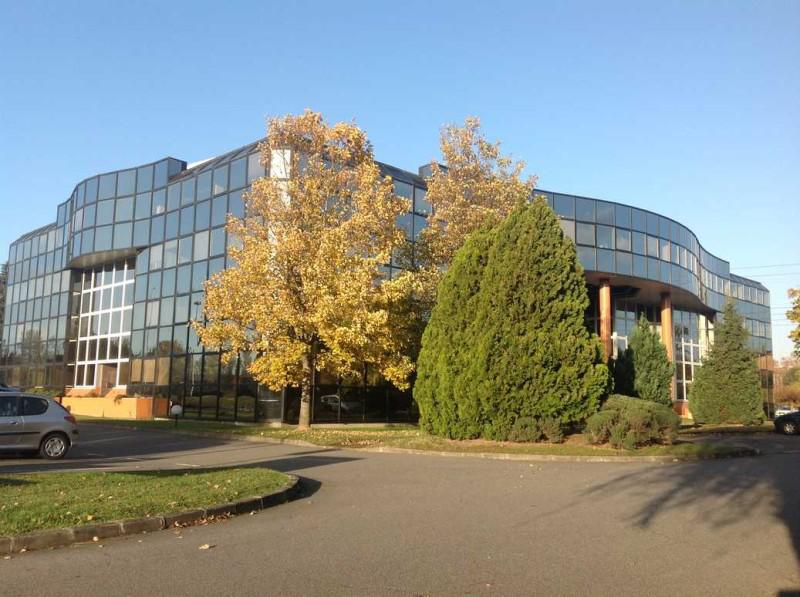
\includegraphics[scale=0.3]{img/bureau.jpg}
    \caption{Batiment Innopolis à Labège(31) où se situe Tachysséma Développement }
    \label{fig:CameraCmdsettings}
\end{figure}



Dans le cadre du master SME, je réalise ma première année d'alternance au sein de la SARL TACHYSSEMA DEVELOPPEMENT basée à Labège (31).
Cette société est impliquée dans des projets en lien avec le traitement vidéo et le traitment du signal en temps réel pour des systèmes éléctroniques embarqués. 

En conséquence, la société possède un rayon d'action étendu qui comprend de la R\&D, du développement matériel (caméras embarquées, conception de cartes éléctroniques) et du dévellopement logiciel. La société est notament spécialisée dans le développement de solutions basées la technologie FPGA.  

Les domaines d'applications de la société sont également variés puisque la société peut être amenée à réaliser des projets pour les secteurs de l'aéraunotique, médical, militaire ou encore automobile. 



\subsection{Organisation interne}

Les locaux de Tachysséma Développement sont partagés avec Visif Technology, une société spécialisée dans le dévellopement de solutions technologiques pour les énergies renouvelables. Cependant les deux sociétés possèdes des projets communs et coopèrent ensembles sur ces projets. 

Au sein de Tachysséma Développement, Nicolas Roddier, mon tuteur d'alternance et gérant de la société est assité par un ingénieur automaticien ainsi qu'une stagiaire en M2 SME, un alternant en M2 SME et moi même. 





\newpage

\section{Projets Réalisés}
Dans cette partie nous réaliserons la synthése des projets principaux menés depuis mon arrivée chez Tachysséma Développement, en septembre 2019. 

\subsection{Réalisation d'une IHM avec l'environnement GTK}

Dans le cadre d'un projet de gestion et contrôle de pixels deffectueux présents sur un capteur d'une caméra, j'ai réalisé une interface homme machine permettant de réaliser l'interface entre l'utilisateur et un module FPGA qui contrôle le capteur d'une caméra. 
\\ 

\subsubsection{Contexte} 

Le capteur d'une caméra est constitué d'un ensemble pixels qui captent la lumière entrante. On peut représenter l'ensemble de ces pixels sous la forme d'une matrice. Avec le temps, il est possible que certains pixels deviennent deffectueux, on parle alors de pixels morts. Les pixels deffectueux doivent pouvoir être localisés, corigés ou remplacés.  
\newline

La caméra est composée d'un FPGA qui contrôle le capteur vidéo. Il permet notament de réaliser le traitement des pixels deffectueux. L'interface homme machine interragit avec le FPGA, elle permettra la réalisation d'actions de lectures et d'écriture dans une table qui contient les coordonnées matricielle des pixels morts. 

\subsubsection{Cahier des charges de l'IHM } 

\begin{figure}[ht]
	\centering
    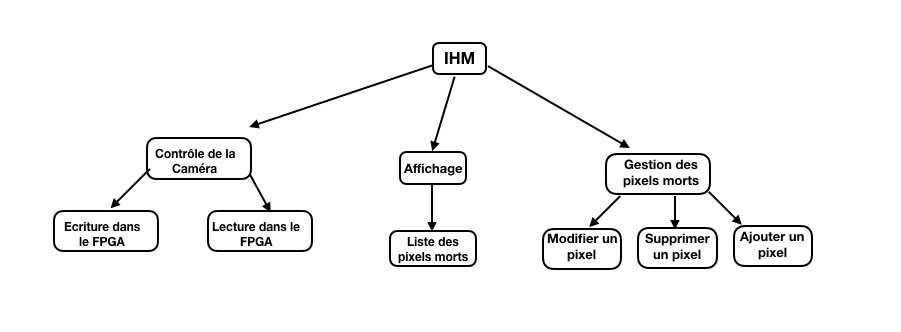
\includegraphics[scale=0.5]{img/cdcIHM.png}
    \caption{Générateur MAVGEN}
    \label{fig:mavgen}
\end{figure}

Voici ci-dessous les principales fonctions qui sont réalisées par l'IHM : 
\newline
\begin{itemize}
	\item L'utilisateur peut lire et écrire la liste des pixels déffectueux dans un fichier .txt qui est sauvegardé sur le disque dur de l'ordinateur (où est executée l'IHM). 
	\item L'IHM peut intérragir avec la caméra par le biais d'une communication série. Elle réalise des opérations de lectures et d'écritures dans une table FPGA ainsi que dans une mémoire EEPROM qui contient les coordonnées des pixels défectueux. 
	\item Une fois que les coordonnées des pixels morts sont chargées de la caméra vers l'IHM ou du fichier .txt vers l'IHM, cette dernière les affiches sous la forme d'une liste comportant deux colonnes (une pour la ligne et une pour la colonne du pixel mort). 
	\item L'utilisateur peut effectuer différentes actions sur la liste des mauvais pixels. Il peut notament ajouter, supprimer ou remplacer des pixels deffectueux. A chaque modification, la liste est actualisée et transmise au FPGA.

\end{itemize}

\subsubsection{Implémentation}

\begin{figure}[ht]
    \centering
    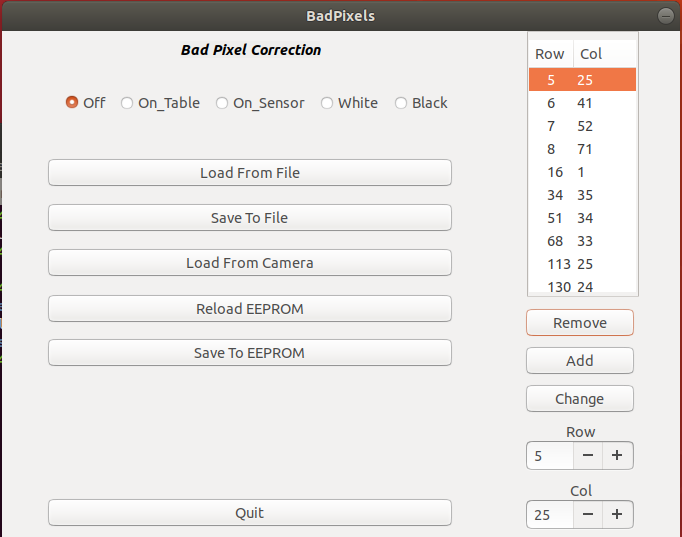
\includegraphics[scale=0.45]{img/IHM.png}
    \caption{Apperçu de l'IHM}
    \label{fig:CameraCmdsettings}
\end{figure}

\subsubsubsection{Interface graphique}

La première étape que j'ai effectué sur ce projet est la réalisation de la partie graphique de l'IHM. Cette dernière devait s'éxecuter sur une distribution linux.

En conséquence j'ai utilisé l'outil de développement graphique Glade qui intègre GTK+. Glade permet facilite la réalisation d'interfaces graphiques: En effet le développeur vient placer les différents objets ( boutons, champs de texte, curseurs etc .. ) sans passer par le code. 

Une fois ce processus terminé, glade génrère la solution obtenu dans un fichier .XML que nous pouvons intégrer directement dans un langage de programmation ( C, C++, Pyhton et d'autres encore). 
\newline

\subsubsubsection{Implémentation du code}

Ensuite j'ai pu implémenté le code en langage C qui permet d'établir un lien entre un évement lié à l'interface graphique ( appuie sur un bouton, changement de valeur sur un curseur ..) et une fonction répondant au cahier des charges ( envoie des données dans le FPGA, quitter l'IHM ou encore écrire le fichier .txt par exemple). 



\subsection{Projet WindFloat Atlantic : Traitement des données d'un équipement embarqué}

\begin{figure}[ht]
    \centering
    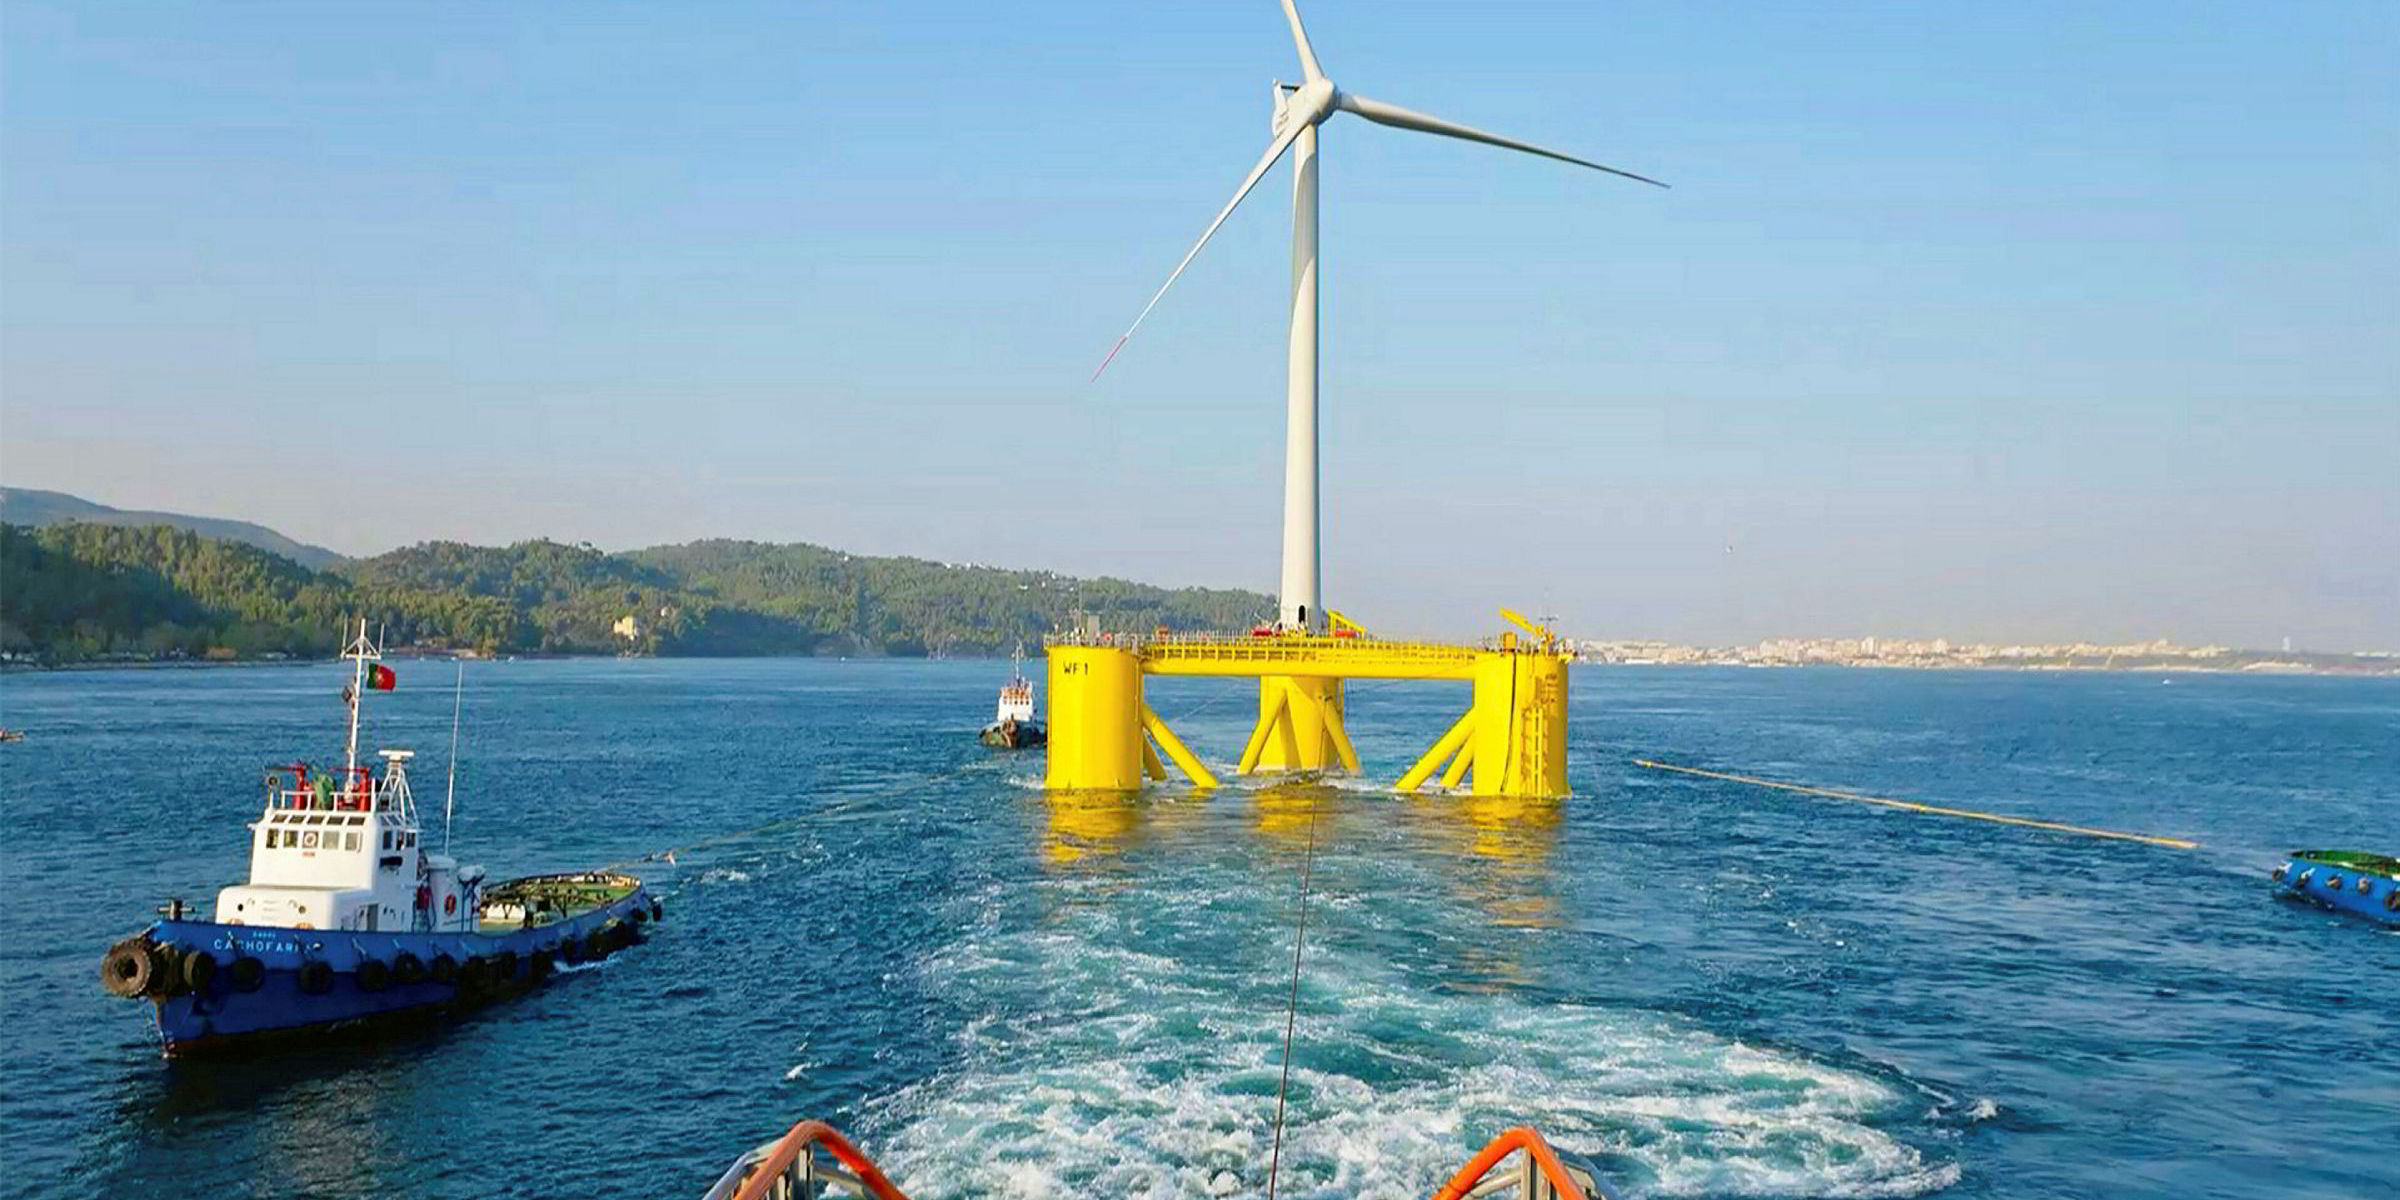
\includegraphics[scale=0.15]{img/WindFloatProject.jpeg}
    \caption{Plateforme située au Portugal}
    \label{fig:CameraCmdsettings}
\end{figure}

\subsubsection{Contexte}
\subsubsubsection{Le projet WindFloat Atlantic}

Tachyssema Developpement participe au projet WindFloat Atlantique mené par EDP Renewables, Engie, Repsol et Principle Power Inc. Ce projet de grande ampleur consite à la réalisation de plateformes exploitants l'énergie éolien offshore.

"WindFloat permet de développer des ressources énergétiques dans de vastes zones marines et de relever des défis majeurs, tels que la transition vers le zero carbone, la sécurité énergétique et la lutte contre le changement climatique, tout en créant des emplois, une croissance économique et des opportunités pour des investissements durables." (source : www.engie.com )

\subsubsubsection{Traitement des données utile pour l'asservissement d'une plateforme}
Informations utiles: Le Xsens MTi-10-series est un module qui regroupe un ensemble de capteurs permettant d'obtenir des informations d'une grande précision sur l'orientation, l'inclinaison, les accélérations sur 3 axes ( x,y,z) ainsi que les positions GPS. 
\newline

Les plateformes sont équipés d'un asservissement leurs permettant de rester stables malgrès des conditions métérologiques pouvant être difficiles comme dans le cas d'une forte houle ou de vents trop importants. Les plateformes sont équipés de trois flotteurs qui assurent leurs bon équilibre. Des pompes à eau sont présentes dans chaque flotteur. L'asservissement agit sur la commande de ces pompes à eau pour maintenir les plateformes en équilibres. 

La positions GPS doivent aussi être connu en temps réel pour vérifier que les plateformes ne dérives pas. 
Toutes ces données proviennent de modules Xsens installés directement sur les plateformes qui transmettent les informations par communication série à un automate qui est lui même relié au sol par via le protocole de communication MODBUS.  (voir figure ci-dessous)
\newpage


\begin{figure}[ht]
    \centering
    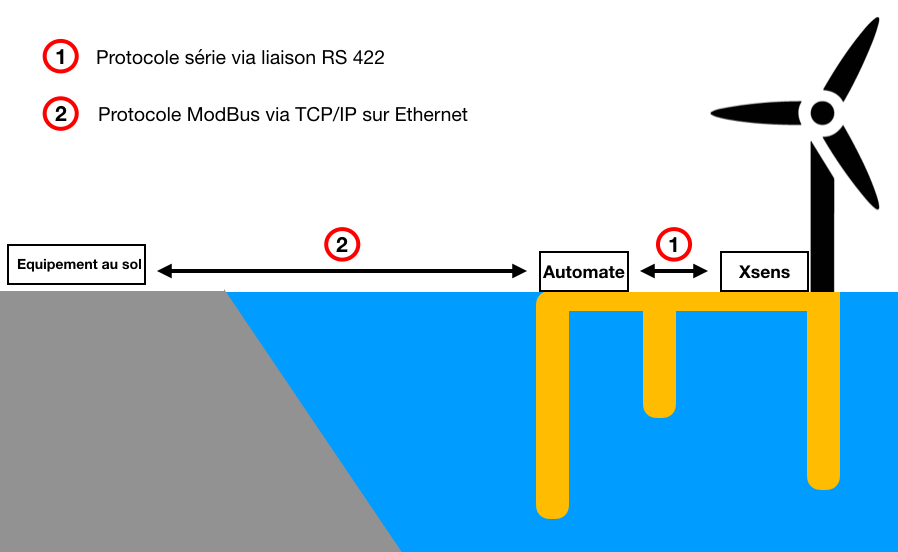
\includegraphics[scale=0.45]{img/schKOWL.png}
    \caption{Illustration de la communication entre équipements }
    \label{fig:CameraCmdsettings}
\end{figure}

\subsubsection{Travail effectué}

Ma mission sur ce projet consistait à : 

\begin{itemize}
	\item Configurer le module Xsens pour que les données répondants au cahier des charges soient transmises à la bonne fréquence ( qui était initialement de 50 Hz). Les données utiles étaient donc le lacet (yaw), le roulis (roll), le tangage (pitch), la lattitude, la langitude ainsi que les accélérations X,Y et Z. 
	\item Etudier la trame générée par le module Xsens, le fonctionnement de la réception série de l'automate et la transmission des données en provenance de l'automate via le protocole MODBUS. 
	\item Créer un executable en C\# (s'exécutant sur un équipement au sol) permettant de lire les données disponibles sur l'automate, de les interpréter pour reconstituer la trame du module Xsens et enfin d'extraire les informations souhaitées. 

\end{itemize}

\subsection{Etude du protocole MAVLINK }

\subsubsection{Contexte}

Le protocole MAVLINK est un ...


\newpage

\section{Présentation de mon projet de M2 }

Dans cette partie nous nous interesserons à mon projet de deuxième année d'alternance que je commence à mener dès cette année en parallèle de mes autres projets en cours. 

\subsection{Présentation}

Mon projet de M2 consiste à la réalisation d'un boitier compatible avec les rails DIN, intégrant un FPGA permettant de réaliser diverses opérations de traitements. L'objetif fixé est de concevoir la carte PCB qui acceuillera les élements électroniques ainsi que la partie mécanique qui correspond au boitier tout en répondant à toutes les normes en vue d'une commercialisation sur le marché. 

\subsection {Pourquoi réaoiser ce projet ? } 

L'interêt de la mise en oeuvre d'un tel boitier est de pouvoir répondre à un besoin client important. En effet ce boitier pouvant s'adapter sur un rail DIN pourra être utilisé pour réaliser des opérations (traitement vidéo, calculs spécifiques ..) que les autres équipements ne peuvent pas réaliser.

Par exemple si on prend le cas d'un automate qui possède une puissance de calculs limitée. Les données à traiter sont transmises au boitier contenant le FPGA, traitées puis renvoyées dans l'automate. 

\subsection {Cahier des charges } 

Le projet doit répondre à un cahier des charges précis : 
\newline
\begin{itemize}
	\item Le boitier doit être compatible avec les rails DIN.
	\item La carte pcb doit être optimisée pour le boitier. Les contours de la carte seront établis en fonction de la forme du boitier.
	\item La carte électronique pourra être programmée par le biais d'un port USB.
	\item La carte électronique disposera de 4 connecteurs SFP qui pourront servir d'entrées ou de sortie.
	\item Le projet devra répondre au normes de comptatibilités électroniques.
	\item Le projet devra répondre au normes CE en vue d'une commercialisation. 

\end{itemize}


\subsection {Réalisation du boitier } 

Dans un premier temps j'ai commencé la réalisation du boitier qui acceuillera la carte pcb. Phoenix Contact est un fabriquant de solutions industrielles qui propose également un service de personnalisation de boitier industriels. Ce service laisse un libre choix aux clients en ce qui concerne les types de boitiers souhaités, les dimensions du boitier ainsi que le choix des connecteurs utilisés.
\newline
Dans un premier temps, j'ai donc réalisé sur le site de Phoenix Contact un boitier compatible rail DIN répondant au exigences du cahier des charges. Une fois la configuration terminée, Phoenix Contact fournit le modèle 3D du boitier : 
\newpage
\begin{figure}[ht]
    \centering
    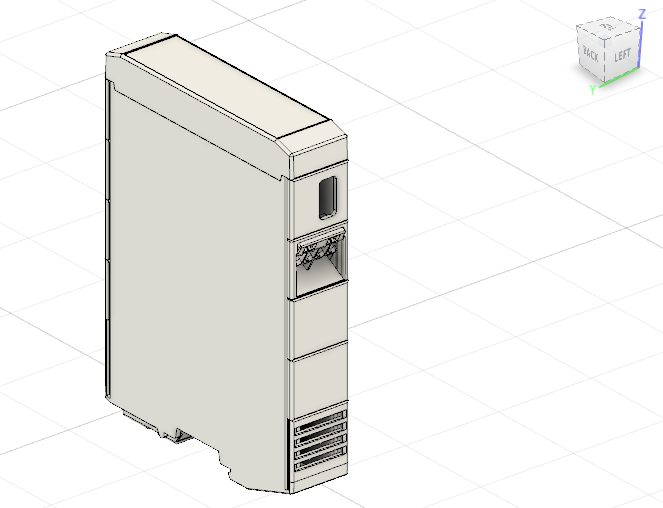
\includegraphics[scale=0.35]{img/boitier.PNG}
    \caption{Apperçu de la conception 3D du boitier }
    \label{fig:CameraCmdsettings}
\end{figure}

On peut également voir que les contours de la carte PCB sont eux aussi générés par le site web : 

\begin{figure}[ht]
    \centering
    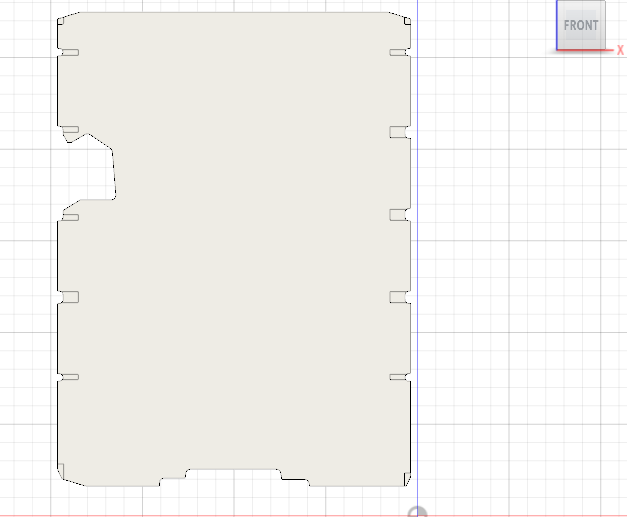
\includegraphics[scale=0.45]{img/pcb.PNG}
    \caption{Apperçu de la conception 3D du boitier }
    \label{fig:CameraCmdsettings}
\end{figure}




\clearpage

\end{document}